\problemname{Astronom}
\illustration{.3}{img/TychoBrahe.JPG}{}

\noindent
Die Leidenschaft unseres Astronoms ist die Sternbeobachtung.
Insbesondere macht es ihm große Freude, $k$~Sterne gleichzeitig durch sein Teleskop zu betrachten.   
Der Bau eines Teleskops mit Radius~$r$ kostet $t\cdot r$~Kronen.
Ein neu gebautes Teleskop wird genau auf den Ursprung $(0,0)$ zeigen.
Es an einen anderen Ort zu verschieben kostet ebenfalls Mühe:
Die Verschiebung des Teleskops um eine Entfernung von $d$~Einheiten verursacht Kosten von $s\cdot d$~Kronen.
Der Astronom kann alle Sterne beobachten, die höchstens $r$ von der Stelle entfernt sind, auf die das Teleskop zeigt.

Wie viel kostet es, ein Teleskop zu bauen und zu bewegen, mit dem $k$~Sterne auf einmal beobachtet werden können?


\medskip

Alle Koordinaten und Entfernungen sind in der euklidischen Ebene angegeben.


\section*{Beispiel}

Hier ist ein Beispiel mit $n=3$ Sternen an den Positionen $(0,0)$, $(2,0)$ und $(3,1)$.
Der schraffierte Bereich zeigt ein Teleskop mit Radius~$1$, das auf $(1,0)$ gerichtet ist und zwei Sterne abdeckt; dieses kostet $s + t$~Kronen und ist eine optimale Lösung für die Beispieleingabe ~$3$.
Das Bild zeigt auch optimale Lösungen für die Beispieleingaben~$1$, $2$, und $4$.

\medskip
\noindent
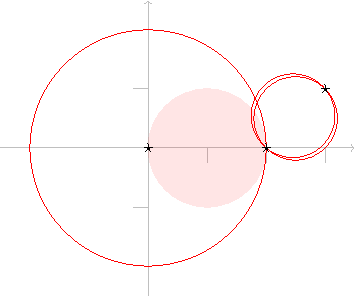
\includegraphics[width=.3\textwidth]{img/samples.pdf}


\section*{Eingabe}

Die erste Zeile besteht aus vier ganzen Zahlen:
die Anzahl~$k$ der Sterne, die der Astronom beobachten will,
die Anzahl~$n$ der Sterne am heutigen Himmel,
die Verschiebungskosten~$s$, und
die Kosten für den Bau des Teleskops~$t$.
Dann folgen $n$ Zeilen, wobei die $i$-te Zeile die ganzzahligen Koordinaten $x_i$ und $y_i$ des $i$-ten Sterns enthält.

\section*{Ausgabe}

Eine einzige reelle Zahl: die Mindestanzahl von Kronen, die der Astronom ausgeben muss.

\section*{Beschränkungen und Bewertung}

Du kannst davon ausgehen, dass 
\begin{enumerate}
\item $1\leq k\leq n\leq 700$. % constraint:kn
\item $x_i, y_i\in \{-10^9,\ldots, 10^9\}$ für alle $i\in\{1,\ldots,n\}$. % constraint:xy
\item $s,t\in \{0,\ldots, 10^9\}$. % constraint:st
\item Deine Ausgabe wird akzeptiert, wenn sie innerhalb einer relativen oder absoluten Toleranz von $\epsilon = 10^{-6}$ der richtigen Antwort liegt.
\end{enumerate}


Deine Lösung wird mit einer Reihe von Testgruppen getestet, von denen jede eine bestimmte Anzahl von Punkten wert ist.
Jede Testgruppe enthält eine Reihe von Testfällen.
Um die Punkte für eine Testgruppe zu erhalten, musst du alle Testfälle in der Testgruppe lösen.
Deine endgültige Punktzahl ist die maximale Punktzahl für eine einzelne Einsendung.

\medskip
\noindent
\begin{tabular}{lll}
  Gruppe & Punkte & Beschränkungen\\\hline
  $1$ & $8$ &  $t\leq s$\\
  $2$ & $9$ & $n\le 50$ und $s=0$\\
  $3$ & $18$ & $s=0$\\
  $4$ & $13$ & $n\leq 50$\\
  $5$ & $14$ & $n\leq 350$\\
  $6$ & $15$ & $\epsilon = 1/10$\\
  $7$ & $23$ & \emph{Keine weiteren Beschränkungen}\\
\end{tabular}
